%%%%%%%%%%%%%%%%%%%%%%%%%%%%%%%%%%%%%%%%%%%%%%%%%%%%%%%%%%%%%%%%%%%%%%%%%%%%%%%
\chapter{Results}
\ifpdf
    \graphicspath{{Chapter4/Figs/Raster/}{Chapter4/Figs/PDF/}{Chapter4/Figs/}}
\else
    \graphicspath{{Chapter4/Figs/Vector/}{Chapter4/Figs/}}
\fi

This chapter examines some of the main results encountered from application of
\textbf{Frontier} and \textbf{scikit-learn} to the task of replicating
classification results from the current \textbf{auto\_qc} system.
Following this chapter, Part II will begin exploring the effects lanelet quality
carries to downstream variant calling analysis.

\section{Introduction}
\subsection{Objectives}

The investigation considers of the following main objectives:

\begin{itemize}
    \item Outline some parameter sets for initial examination
    \item Use parameter selection for more rigorous modelling
    \item Attempt to minimise generated trees
    \item Investigate application of best practice for tree construction
    \item Identify particular parameters that are of use for classification
\end{itemize}

\subsection{Decision Trees}
%TODO Citations...

A \textbf{decision tree} is a structure of \textbf{nodes} where each node
represents a test on the value of a particular feature or parameter of an
observation. The layout of a decision tree resembles a flow chart where
'decisions' at each node (\textit{e.g.} is parameter x greater than or equal to
value y) choose the path an observation will take through the tree. Once an
observation has reached a \textbf{leaf} node -- a node with no test to be
applied -- it is considered classified (typically the leaf will either be
trained to contain observations of just one class, or the classification will be
the most frequent class in that leaf).

Our primary motivation for using a decision tree is its interpretability; trees
create human-readable rule sets and are very easy to explain and understand. The
current \textbf{auto\_qc} system performs logical tests of simple rules in a
similar fashion and thus it seemed sensible to compare results from both systems
by using a decision tree as output. A "black box" machine learning
classifier such as a neural network would not produce any tangible rules that
could be explained to another human. Whilst the first goal is to briefly
investigate whether \textbf{auto\_qc}'s rules actually can be recovered, future work may
wish to make improved rules that could still be interpreted by lab technicians,
which would be impossible with a "black box" algorithm.

%TODO Cite robustness
Decision trees are robust to noise and missing data (within reason) and can be
realistically deployed in a variety of applications including medicine and
finance. Decision trees also scale well to large inputs, which is useful given
the size of the data set (approximately 1.15 million observation-parameter
combinations).

%TODO Cite cross val, cite overfitting
However, trees are prone to a process called \textbf{overfitting}, where
decisions have too much basis on the data seen so far and don't generalise well
to future observations. \textbf{Cross-validation} can help overcome this barrier
by splitting the available data and targets into training and testing subsets.
The tree will be constructed using the training set and the accuracy of the tree
is then measured on the unseen testing data (\textit{i.e.} did classifications
made by the tree match the known targets for those observations?).

\section{Interaction with scikit-learn}
\subsection{DecisionTreeClassifier}
% TODO Cite
% http://scikit-learn.org/stable/modules/generated/sklearn.tree.DecisionTreeClassifier.html

\textbf{scikit-learn} provides the \textbf{DecisionTreeClassifier} class as an
interface to creating decision tree objects. 

...gini impruty or information gain... scikit seems to favour gini...
...
...Classification And Regression Tree (CART)


\subsection{Cross Validation}

...method in which to measure classification accuracy...
...potentially use a weighting to penalise mistakes in smaller classes...

...K fold cross validation
...using stratified K fold cross validation...


\subsection{Confusion Matrices}
"Normal" confusion matrix and "Warnings" confusion matrix...


\section{Naive Parameter Sets}
\subsection{Introduction}

For initial training and testing purposes, the following arbitrary parameter
sets were created as a starting point:

\begin{itemize}
    \item \textbf{ALL} \hfill\\
        A parameter set consisting of all the summary numbers in a "BAMcheckr'd"
        file
    \item \textbf{AQC} \hfill\\
        A set consisting of all available parameters used by \textbf{auto\_qc}.
    \item \textbf{AQCN} \hfill\\
        Replaces groups of the \textbf{AQC} set with aggregated parameters.
    \item \textbf{ERROR} \hfill\\
        An experimental toy set consisting of only the "error-rate" parameter.
    \item \textbf{NO\_ERROR} \hfill\\
        Another toy set designed to test results gained by excluding the
        "error-rate" parameter.
    \item \textbf{BASELINE} \hfill\\
        Include any parameter which includes "baseline" as a substring.
    \item \textbf{NOBASELINE} \hfill\\
        Exclude any parameter which includes "baseline" as a substring.
    \item \textbf{MARP} \hfill\\
        Include any parameter which includes any of the following as substrings:
        mean, average, rate or percent.
    \item \textbf{NO\_MARP} \hfill\\
        Exclude any parameter which includes any of the following as substrings:
        mean, average, rate or percent.
\end{itemize}

Of particular note is the \textbf{AQC} set, constructed from the parameters
available from the "BAMcheckr'd" data that are taken into account by the
current \textbf{auto\_qc} system. However not all these
parameters were initially available in the input files and \textbf{auto\_qc}
relies upon data made available from \textbf{vr-pipe} where the rules of
\textbf{auto\_qc} are actually applied; Appendix~\ref{app:ratios} discusses
contributions I made to \textbf{bamcheckr} for recovering these parameters for
use in our analysis. Ultimately, \textbf{bamcheckr} performed too slowly and it
was possible to use \textbf{Frontier} itself to extract the additional features
needed to better represent the decisions made by the current system.

\subsection{Experiment Results}
%TODO Cite dtc, skfold
For each parameter set, data and targets were extracted via \textbf{Frontier}'s
API before being subset by \textbf{scikit-learn}'s \textbf{StratifiedKFold}
function. All available data (13,455 "BAMcheckr'd" lanelets) were used as input
and the target variable could be one of three classes; pass, fail or warn.
The subsets are referred to as "folds" (of which we used 10) and for
each fold a \textbf{DecisionTreeClassifier} was trained and tested.
Table~\ref{tab:pset-cv} outlines the average cross validation scores across each
such experiment.

\begin{table}
    \centering
    \begin{tabular}{l | c  c  c  c  r}
        Set           & Nº & CV ± SD & SCV ± SD & Depth & Most Important Feature\\
        \hline
        ALL           & 86 & 90 ± 4 & 97 ± 1 & 38 & T-percent-max-baseline-deviation (27\%)\\
        AQC           & 27 & 87 ± 4 & 95 ± 1 & 36 & T-percent-max-baseline-deviation (31\%)\\
        AQCN          & 21 & 86 ± 4 & 95 ± 1 & 39 & max-max-baseline-deviation (31\%)\\
        ERROR         & 1  & 60 ± 6 & 61 ± 2 & 53 & error-rate (100\%)\\
        NO\_ERROR     & 85 & 90 ± 4 & 97 ± 1 & 38 & T-percent-max-above-baseline(27\%)\\
        BASELINE      & 34 & 82 ± 5 & 89 ± 1 & 46 & T-percent-max-above-baseline(28\%)\\
        NOBASELINE    & 52 & 72 ± 10 & 91 ± 1 & 31 & error-rate (24\%)\\
        MARP          & 47 & 87 ± 4 & 95 ± 1 & 39 & T-percent-max-above-baseline (27\%)\\
        NO\_MARP      & 39 & 75 ± 7 & 87 ± 1 & 38 & max-max-baseline-deviation (34\%)\\
    \end{tabular}

    \caption[pset-cv]{\textbf{Parameter Set Cross Validation Scores}: Results of
        classifying testing data into one of three classes; pass, fail or warn.
        Columns left to right; parameter set name, number of parameters
        included, average cross-validation score (max 100) ± std. deviation,
        average stratified cross-validation score (max 100) ± std. deviation,
        average depth of the generated tree and the most important parameter by
        Gini importance (max 100). Tree depth and parameter importance was
    estimated on experiments using the stratified data.}

    \label{tab:pset-cv}
\end{table}

Whilst these parameter sets are certainly crude -- a majority of them having
been constructed without close examination just by matching or excluding
substrings using \textbf{Frontier}'s parameter inspection functions -- we can
learn quite a lot about the available data.

Firstly it should be of no surprise that the \textbf{ALL} model scores highly in
both cross-validation and stratified cross-validation testing. The feature group
is a superset over the same parameters used by \textbf{auto\_qc} itself.
Similarly the \textbf{NO\_ERROR} set which uses all but one parameter
(\textbf{error-rate}) scores highly.

It's interesting to compare the scores between the \textbf{AQC} and
\textbf{AQCN} parameter sets against \textbf{ALL}. Both of the former score
highly despite having significantly fewer parameters. This appears to indicate
that many of the parameters in the \textbf{ALL} model are redundant for use in
classification. This should of course be expected; you'd hope to see that a set
that includes parameters known to be used by the current \textbf{auto\_qc} system
is capable of replicating results made by that system.

In general the other models perform reasonably well, potentially reflecting the
simple linear nature of the decisions made by the \textbf{auto\_qc} system.

Stratified cross-validation scores are consistently better and less variable
(smaller standard deviations) than their non-stratified counterparts. This
should be due to the more "balanced" training and testing sets
gained by assigning observations to folds to match their proportions in the
whole data set. The differences between the pairs of validation scores is
predictable -- averaging 8.66 percentage points -- but the \textbf{NOBASELINE}
set presents a difference of almost 20pp and exhibits more variable behaviour.
This suggests that excluding the baseline related parameters is problematic for
one (or two) of the three class labels (as the only difference expected between the
experiments will be the proportions of the classes).

The average maximum tree depth -- ranging between 31 and 53 splits -- may be
highlighting a possible shortcoming of using a decision tree classifier;
complexity could be indicative that a tree may have been overfitted on the training
data. Later sections will apply best practice in an attempt to minimise this
effect.

%TODO Gini importance
Whilst \textbf{T-percent-max-baseline-deviation} is a parameter used by
\textbf{auto\_qc}, it was not believed to be a parameter of
particularly major importance and yet it is ranked as the \textit{Most
Important Feature} by \textbf{scikit-learn}'s feature importance algorithm
for all parameter sets it was a member of. Further investigation will yield a
more authoritative conclusion as to whether the influence of this parameter
should be reassessed.


\subsection{Summary of Trees}

Figures~\ref{fig:all-all-1} and~\ref{fig:all-all-2} are two of the ten trees
constructed (one per fold) during the testing of the \textbf{ALL} paramter set.
The breadth and depth of the trees are somewhat reasonable and stand up to
scrutiny by cross validation (stratified or not). The depth of the trees appear
to be a result of a paticular decision path consisting of a large number of
observations passing through nodes and splitting off a small subset of
observations each time, akin to a busy train dropping small groups of
passengers off at small stations. This linear behaviour matches the role of
\textbf{auto\_qc}...



\begin{figure}[htbp!]
    \centering
    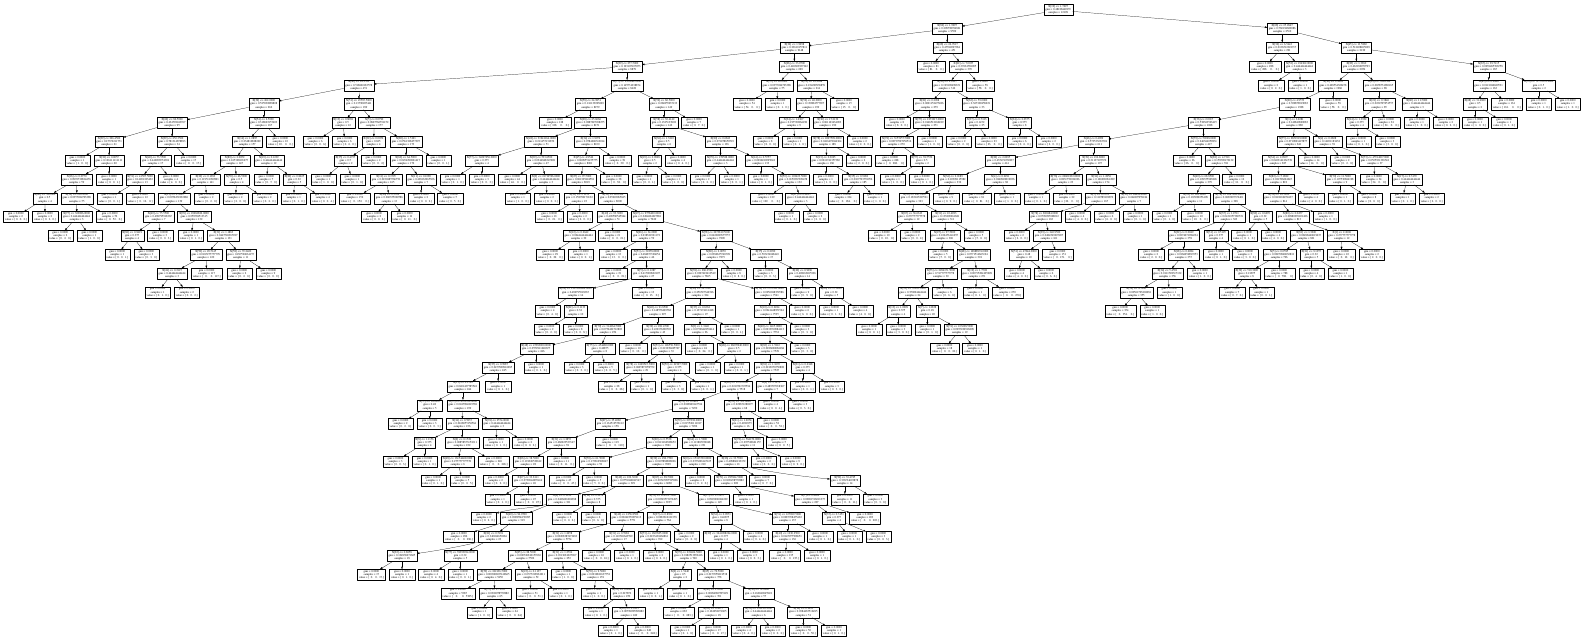
\includegraphics[width=1\textwidth]{ALL_ALL_1}
    \caption[all-all-1]{\textbf{ALL Set Decision Tree A}}
    \label{fig:all-all-1}

    \vspace{20mm}

    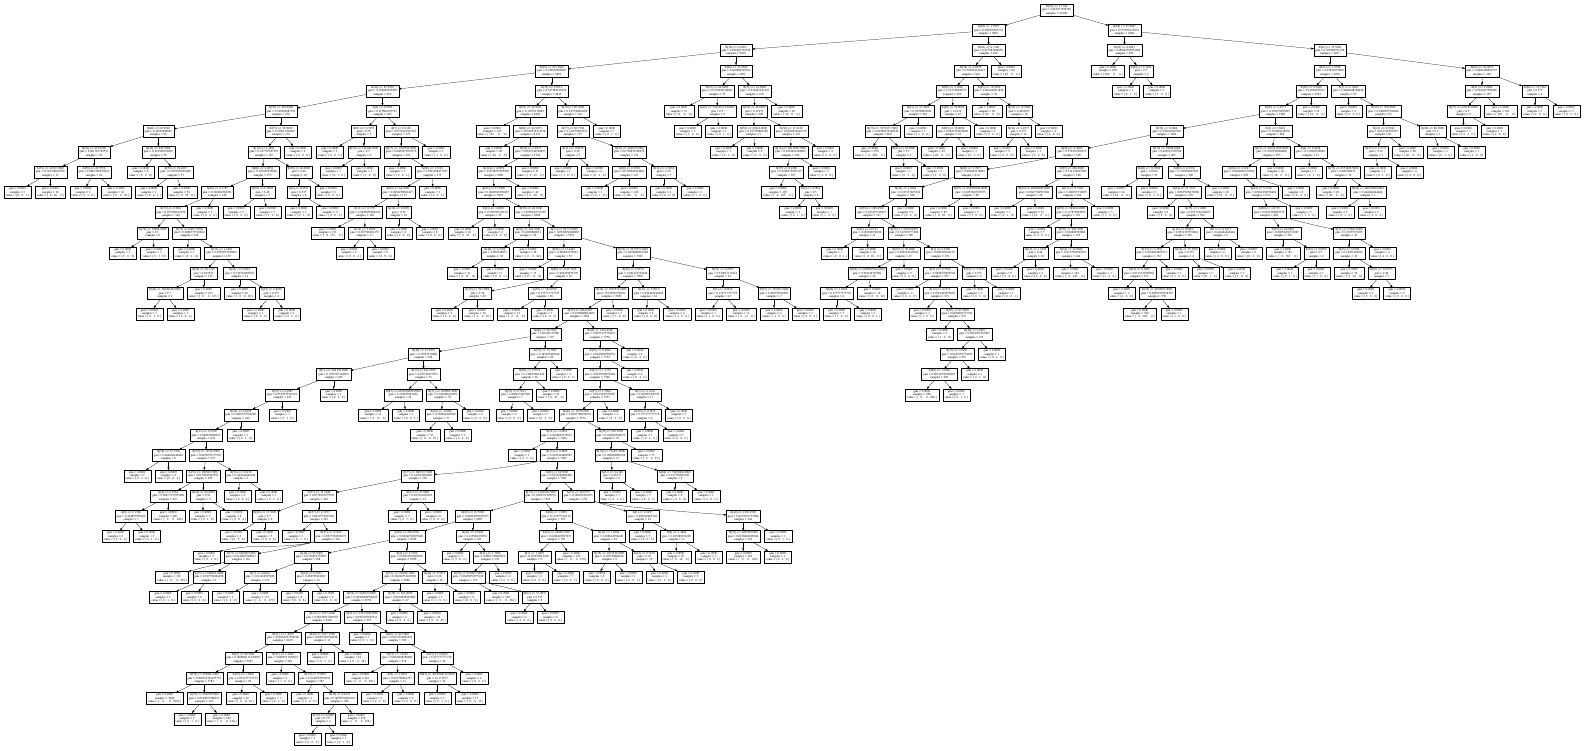
\includegraphics[width=1\textwidth]{ALL_ALL_2}
    \caption[all-all-2]{\textbf{ALL Set Decision Tree B}}
    \label{fig:all-all-2}
\end{figure}

Figures~\ref{fig:all-aqc-1} and~\ref{fig:all-aqc-2} are two of the ten trees
generated via training and testing of the significantly smaller \textbf{AQC}
parameter set. Whilst the size of these trees has grown (though the average
depth for the \textbf{AQC} set is in fact lower than \textbf{ALL}), they also
exhbit the linear \textbf{auto\_qc} behaviour.

It is interesting to note the apparent difference in size between these two
trees, although they were generated using parameters from the same set, the
results of training the trees are more variable. This could hint that there are
parameters we have excluded (that are present in \textbf{ALL}) that may
be useful in maintaining tree stability.

\begin{figure}[htbp!]
    \centering
    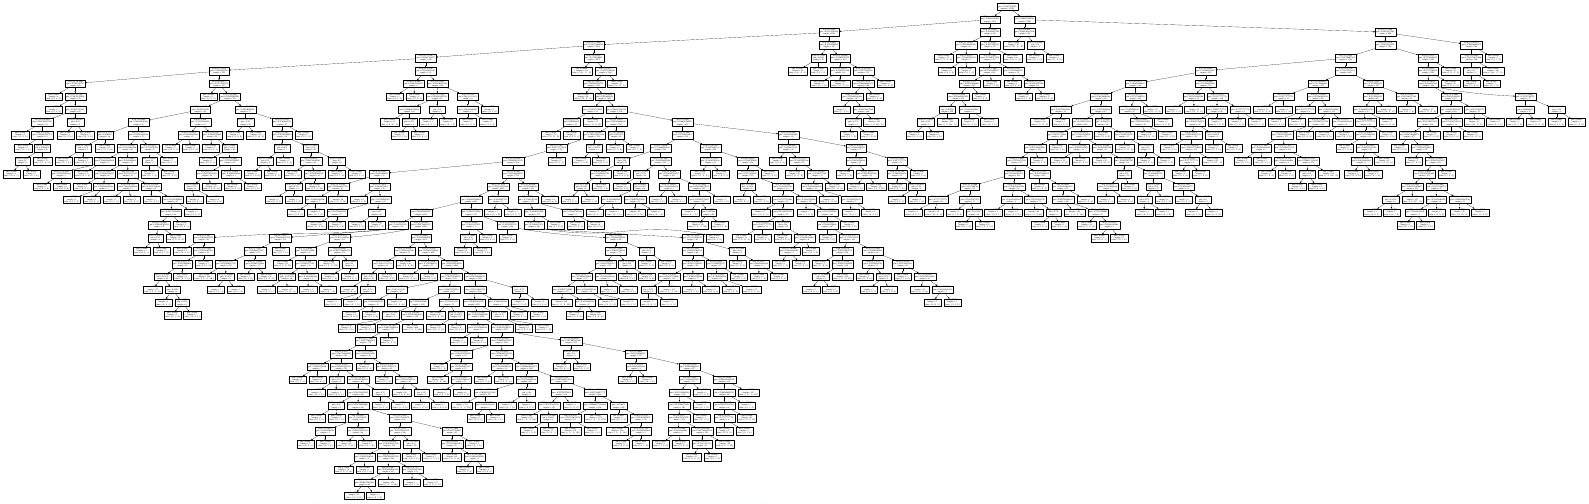
\includegraphics[width=1\textwidth]{ALL_AQC_1}
    \caption[all-aqc-1]{\textbf{AQC Set Decision Tree A}}
    \label{fig:all-aqc-1}

    \vspace{20mm}

    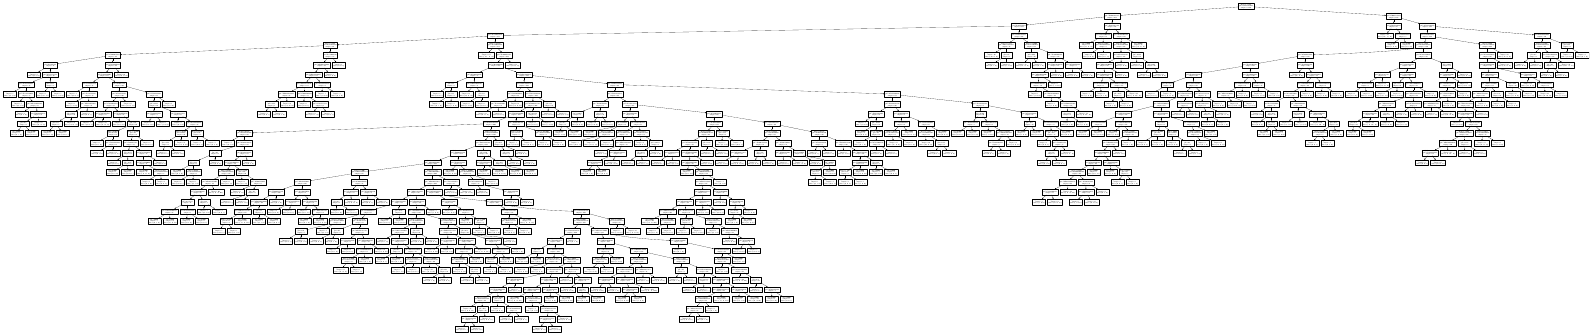
\includegraphics[width=1\textwidth]{ALL_AQC_2}
    \caption[all-aqc-1]{\textbf{AQC Set Decision Tree B}}
    \label{fig:all-aqc-2}
\end{figure}


Figures~\ref{fig:all-baseline-1} and~\ref{fig:all-error-1} are examples of
poor decision trees. Splitting decisions are overly complicated, creating an
uninterpretable sprawl of nodes and leaves. Rules will be incredible difficult
to extract, if not impossible and will be very unlikely to offer any real
meaning. Figure~\ref{fig:all-error-1} in particular is a highly overfit tree,
constructed on just one parameter (\textbf{error-rate}); every node in the tree
is an arbitrary decision, classifying the trained observations exactly.

The \textbf{ERROR} set however acheives a cross-validation score of 60\%,
highlighting the necessity of examining created trees and not just blindly
accepting the validation scores. Despite its somewhat acceptable performance
(60\% accuracy in a three class problem), no
useful rules can be extracted. In addition, you would require a 42m wide
wall to hang it on if you wanted a handy classification guide in a lab.


\begin{sidewaysfigure}[htbp!]
    \centering
    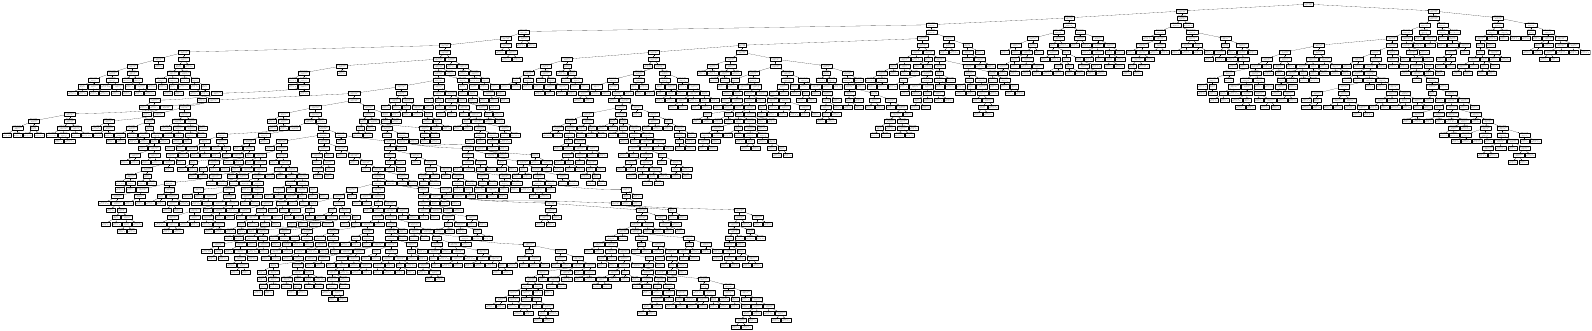
\includegraphics[width=\textheight,height=4cm]{ALL_BASELINE_1}
    \caption[all-baseline-1]{\textbf{BASELINE Set Decision Tree}: A
    decision tree trained using the \textbf{BASELINE} set.}
    \label{fig:all-baseline-1}

    \vspace{20mm}

    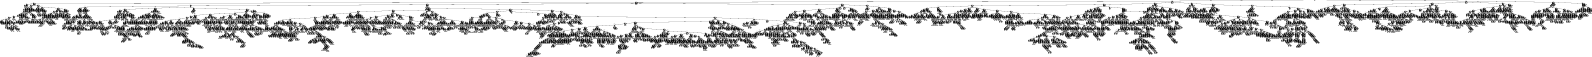
\includegraphics[width=\textheight,height=1cm]{ALL_ERROR_1}
    \caption[all-error-1]{\textbf{ERROR Set Decision Tree}: A highly
        overfit decision tree trained on the single parameter \textbf{ERROR}
    set.}
    \label{fig:all-error-1}
\end{sidewaysfigure}


\section{Informed Parameter Selection}
\subsection{Introduction}

Whilst the crude parameter sets of the previous section were useful to gain
understanding of the data that we have, it was necessary to obtain more
deliberate decisions for parameters to utilise in the model.

\textbf{Frontier} uses two methods for the selection of 'best' parameters:

\begin{itemize}
    \item Backward elimination; pruning parameters with the lowest total gini
    \item Call scikit-learn's SelectKBest
\end{itemize}

...important to find the "best" parameters
...what is best? scikit-learn uses total gini information

...frontier uses two methods:
\begin{itemize}
    \item Backward elimination; pruning parameters with the lowest total gini
    \item Call scikit-learn's SelectKBest
\end{itemize}

\begin{listing}[H]
    \caption[frontier-warnings]{\textbf{Frontier Variance Warnings}:
        Warnings issued for \textbf{auto\_qc} parameters that have been found to
        have no variance by one of \textbf{Frontier}'s sanity checking procedures.}
    \label{list:frontier-warnings}
    \begin{minted}[mathescape,
                %linenos,
                numbersep=5pt,
                gobble=0,
                frame=lines,
                framesep=2mm]{bash}
/pools/encrypted/sanger/frontier/data/bamcheck_2013dec25_ratios_out/(13455 files)
[WARN] bases-trimmed parameter has 0 variance (with mean 0.00)
[WARN] filtered-sequences parameter has 0 variance (with mean 0.00)
[WARN] is-paired parameter has 0 variance (with mean 1.00)
[WARN] is-sorted parameter has 0 variance (with mean 1.00)
[WARN] maximum-length parameter has 0 variance (with mean 100.00)
[WARN] non-primary-alignments parameter has 0 variance (with mean 0.00)
[WARN] quality-dropoff-high-iqr-threshold parameter has 0 variance (with mean 10.00)
[WARN] quality-dropoff-ignore-edge-cycles parameter has 0 variance (with mean 3.00)
[WARN] quality-dropoff-runmed-k parameter has 0 variance (with mean 25.00)
    \end{minted}
\end{listing}

Parameters with no variance will have constant value across all observations
regardless of their class label and will thus be unhelpful in predicting class
membership for future observations. Such parameters can be safely discarded,
Listing~\ref{list:frontier-warnings} displays warnings issued by
\textbf{Frontier} for several of the \textbf{auto\_qc}


\section{Filtering of Data Sets}

The presentation of data to \textbf{scikit-learn} will greatly influence the
outcome of the classifier. For example, one may choose to determine criteria to identify
outlier observations that will be excluded from a study.

...present here two alternative ways to present our data and targets...

...the \texttt{--d} flag may be used on the \textbf{FrontAQC} script (discussed
previously...) to specify use of one of the sets below... by default it will use
\texttt{--dALL}...

...warnigns no longer exist!

\subsection{Ignoring Warnings}

The aim of \textbf{FrontAQC} is to firstly mimic the \textbf{auto\_qc} system by
training and testing on data sets with known targets as classified by
\textbf{auto\_qc}. However, attempting to learn what \textbf{auto\_qc} doesn't
know might be counter-intuitive. Lanelets are classes as warnings because the
current system doesn't have the rules to mark it otherwise, such classifications
could essentially  be considered as \textbf{auto\_qc} reporting "I don't know".

After manual inspection a lanelet flagged as a warning will be categorised as a
"pass" or "fail" by a human operator. So for all \textbf{Frontier} and
\textbf{scikit-learn} know, a sample with an \textbf{auto\_qc} "warning" could
be eiher a pass or a fail.

In other words, the set of warnings is actually a union between some unknown
subset of the passes and failure. Training on this now seems impractical and
inherently noisy. Users may now specify \texttt{--dIGNWARN} to \textbf{FrontAQC}
to discard all warnings from the data set.


\subsection{Treating Warnings as Passes}

\textbf{auto\_qc}'s rule set is typically able to catch the worst quality
lanelets the system will overcautiously flag other lanelets for manual
inspection. Many of these flagged lanelets are approved after human
intervention, to the degree where by default, lanelets classified with a warning
are allowed to proceed downstream for further analysis -- as if they were a
pass.

If \textbf{auto\_qc} is technically treating warnings as passes, then why
shouldn't we? Thus, using \textbf{Frontier}'s \textit{recode} functionality, a
user may specify \texttt{--dWARNPASS} to \textbf{FrontAQC} to recode all
warnings as passes.


\subsection{Seperating Studies}

%FUTURE
...The "BAMcheckr'd" data set is made up of 13,455 lanelets...
...from two different studies...
...whilst the rule set \textbf{auto\_qc} remained the same for both studies it
would be interesting to investigate whether there are any underlying effects
from study...
Time did not permit exploration of this idea...


\section{Combining Data Filtering and Parameter Selection}

\subsection{Experiment Results}

\begin{table}[H]
    \centering
    \begin{tabular}{l l | c  c  c  c  r}
        PSet & DSet          & Nº & CV ± SD & SCV ± SD & Depth & Most Important Feature\\
        \hline
        RTOP9 & ALL         & 9  & 87 ± 6  & 95 ± 1 & 32 & max-max-baseline-deviation (32\%)\\
        RTOP9 & IGNWARN     & 9  & 98 ± 1  & 99 ± 0 & 20 & rev-pct-insertions-above-baseline (38\%)\\
        RTOP9 & WARNPASS    & 9 & 95 ± 3 & 99 ± 1 & 24 &
                                                    quality-dropoff-rev-mean-runmed\\
                                                    &&&&&&-decline-low-value (34\%)\\
    \end{tabular}

    \caption[pset-cv]{\textbf{Backward Elimination Parameter Set Cross Validation Scores}:
        Results of classifying testing data.
        Columns left to right; parameter set name, data set name, number of parameters
        included, average cross-validation score (max 100) ± std. deviation,
        average stratified cross-validation score (max 100) ± std. deviation,
        average depth of the generated tree and the most important parameter by
        Gini importance (max 100). Tree depth and parameter importance was
        estimated on experiments using the stratified data. \textit{N.B.}
    \textbf{IGNWARN} and \textbf{WARNPASS} data sets perform classifications on
two classes (pass and fail) rather than three.}

    \label{tab:be-pset-cv}
\end{table}
\begin{table}[H]
    \centering
    \begin{tabular}{l l | c  c  c  c  r}
        PSet & DSet          & Nº & CV ± SD & SCV ± SD & Depth & Most Important Feature\\
        \hline
        KTOP9 & WARNPASS    & 9 & 95 ± 3 & . & . & . \\
    \end{tabular}

    \caption[pset-cv]{\textbf{SelectKBest Parameter Set Cross Validation Scores}: Results of
        classifying testing data into one of three classes; pass, fail or warn.
        Columns left to right; parameter set name, number of parameters
        included, average cross-validation score (max 100) ± std. deviation,
        average stratified cross-validation score (max 100) ± std. deviation,
        average depth of the generated tree and the most important parameter by
        Gini importance (max 100). Tree depth and parameter importance was
    estimated on experiments using the stratified data.}

    \label{tab:ks-pset-cv}
\end{table}

\subsection{Summary of Trees}

\begin{figure}[htbp!]
    \centering
    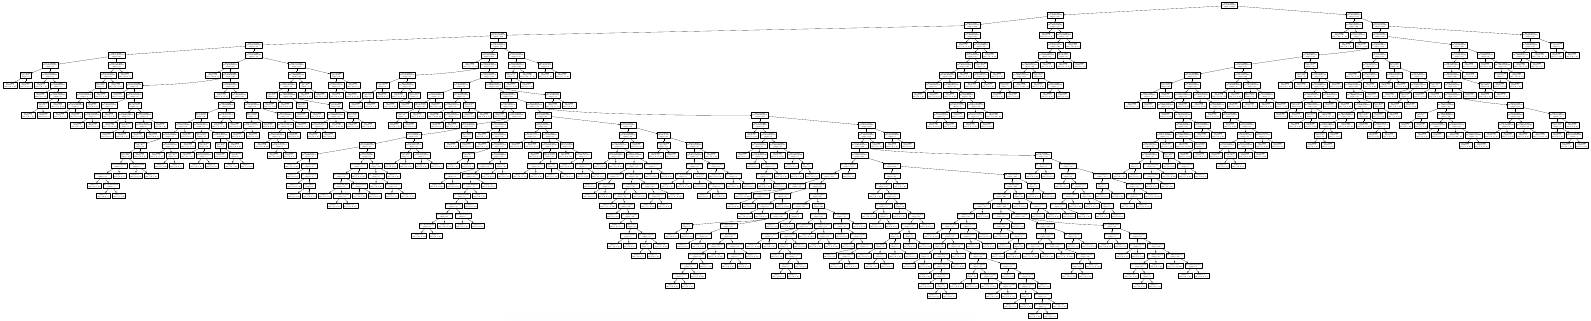
\includegraphics[width=1\textwidth]{TOP9_ALL_1}
    \caption[top9-all-1]{\textbf{TOP9 Set Decision Tree with ALL Data}}
    \label{fig:top9-all-1}
\end{figure}

\begin{figure}[htbp!]
    \centering
    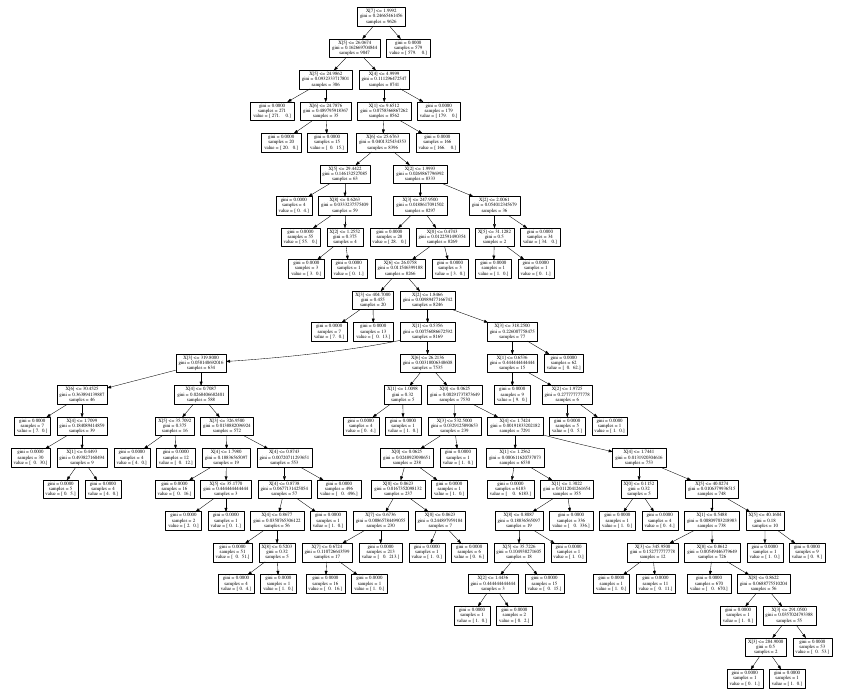
\includegraphics[width=0.8\textwidth]{TOP9_IGNWARN_1}
    \caption[top9-ignwarn-1]{\textbf{TOP9 Set Decision Tree with IGNWARN Data A}}
    \label{fig:top9-ignwarn-1}

    \vspace{10mm}

    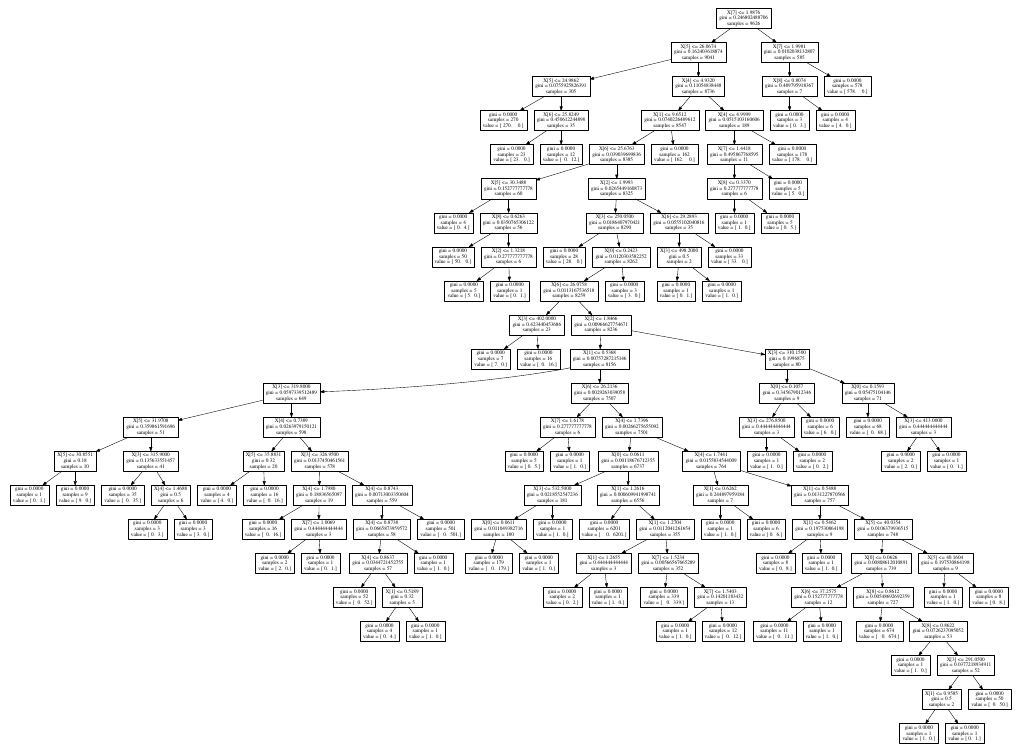
\includegraphics[width=0.8\textwidth]{TOP9_IGNWARN_5}
    \caption[top9-ignwarn-2]{\textbf{TOP9 Set Decision Tree with IGNWARN Data B}}
    \label{fig:top9-ignwarn-2}
\end{figure}


\section{Application of Best Practice}
...scikit has no post pruning...

\textbf{DecisionTreeClassifier} accepts the following optional arguments upon
concstruction:

\begin{itemize}
    \item \textbf{max\_depth} \hfill\\
        Prevent the tree from growing beyond a specified depth.
    \item \textbf{min\_samples\_split} \hfill\\
        Prevent a node in the tree from being split further if it does not
        contain enough observations.
    \item \textbf{min\_samples\_leaf} \hfill\\
        Prevent a node in the tree from being split further if it would create a
        leaf smaller than the required minimum.
\end{itemize}


...
...

* incorrect degrees of freedom
* warnings: /usr/lib64/python2.7/site-packages/sklearn/feature\_selection/univariate\_selection.py:256: RuntimeWarning: invalid value encountered in divide, causing NaN
* Replaced univariate\_selection with version from master
* needed use force np.float64
* ...actually data was 0... gg

\section{Conclusion}

...concludes a brief investigation in to the parameters available...

...able to extract the parameters used...
...cross-validates strongly...

...Part II will undertake an investigation in to lanelet quality...
...locate lanelets that are known to improve or detriment analysis
...and look for patterns in the quality control parameters of these particular
observations to better fuel the search...
